\documentclass[12pt]{article}
\pdfminorversion=7

% Standard packages for figures, citations, math, tables, etc.
% Feel free to add more as needed!
\usepackage{amssymb}
\usepackage{graphicx}
\usepackage{cite}
\usepackage[cmex10]{amsmath}
\interdisplaylinepenalty=2500 
\usepackage{mdwmath}
\usepackage{mdwtab}
\usepackage{color}
\usepackage{pgfplots}
\usepackage{multirow}
\usepackage{subcaption}
\usepackage{verbatim}
\usepackage{enumitem}
\usepackage{appendix}
\usepackage[outdir=./]{epstopdf}
\usepackage{indentfirst}
\pgfplotsset{compat=1.17}

% Packages for formatting with 1 in margins
\usepackage[latin1]{inputenc}
\usepackage[left=1in,top=1in,right=1in,bottom=1in,nohead]{geometry}
\usepackage{setspace}
\setstretch{1.15}
\setlength\parindent{1cm}

% Define the location of your figures in order to avoid writing absolute file location
\graphicspath{{figures/}}	

\begin{document}

% Title Page
\begin{titlepage}
\begin{center}
{\LARGE \textsc{ECE 445: Senior Design Laboratory} \\ \vspace{8pt}}
\rule[13pt]{\textwidth}{1pt} \\ \vspace{120pt}
{\huge \textbf{\textsc{The Odds Booster}} \\ \vspace{8pt}}
{\LARGE \textbf{\textsc{Individual Progress Report}} \\ \vspace{30pt}} 
{\large \textit{Author:} Tim Green \\ \vspace{4pt}
\hspace{8pt} \textit{Date Written:} March 29th, 2022}
\vfill
\end{center}

% Numbered pages on everything but title
\pagenumbering{arabic}	
\end{titlepage}
\setcounter{page}{2}

\section{Introduction}

The Odds Booster is a card game assistant used with Blackjack or Texas Hold'em. These card games can be daunting to new players and this device helps a group or individual learn the game and the value of the different hands. Currently, the main way to learn these games is through being taught by a peer, but our device hopes to make these games more accessible. The device provides instructions for the flow of the game on the main display to help all players learn what to do next at each point in the game. The device also assists an individual player in learning the different hands by pairing to a Bluetooth device and providing an evaluation of the player's hand. The device is able to do all this by reading the cards that are dealt with an RFID scanner on the main device.

The Odds Booster is composed of several subsystems, the power subsystem, the card reader subsystem, the communication subsystem, the display subsystem, and the phone app subsystem. Note that while the phone app subsystem was initially planned to be implemented on an android device, we were unable to acquire one for the course of this project and thus will need to implement it as a windows application. The functionality of the app will remain the same and all of the requirements listed in the design document for the subsystem will still be met. The power subsystem provides a steady 3.3V source to all logic elements in other subsystems and a 9.6V source to the display system for powering the LED backlight of the LCD. The card reader system is an RFID card reader that interacts with the RFID tags on each cards and communicates the card ID to the communication subsystem. The communication subsystem includes the MCU and communicates the card and game information via Bluetooth to the app subsystem. Lastly, the display subsystem is controlled by the MCU within the communication subsystem and shows game information to all players. 

From the start of the project I took responsibility for the design, construction, and verification of the communications and display subsystems. Additionally, I planned on programming the Bluetooth portion of the app subsystem. I have chosen components and designed schematics for the communication and display subsystem. I have created necessary footprints and a layout for the components within these subsystems. As the deadline for the design document approached, my team was not meeting their requirements for their responsibilities so I also chose components and designed schematics for the Low Dropout Linear Voltage Regulator, the Boost Converter, and the Buck Converter within the power subsystem. I have also begun planning the Bluetooth communications implementation for the MCU firmware and the app subsystem.

Moving forward, I plan on constructing the communications and display subsystems by soldering these components to the board. This requires the power system to be constructed and functional first to properly test these subsystems. I plan on completing the firmware of the MCU within the communications subsystem to control the LCD within the display subsystem. I also plan on completing the Bluetooth communication portion of the firmware. For proper functionality of the full system, the MCU requires a successful interface between the RFID reader and itself to be able to accurately receive card IDs. The Bluetooth capabilities can be built before this has been achieved though. Finally, I plan on completing the Bluetooth communication portion of the app subsystem. For proper system operation, the GUI will need to be built to allow users to access the information sent from the central device and to control the device remotely.

\section{Design}

\subsection{Communication Subsystem}

The communication subsystem is primarily composed of the MCU along with some switches and resistors to allow for control and programming of the MCU. The chosen MCU is a ESP32-WROVER-E module which includes an 2.4GHz antenna built into the module. This simplifies the Bluetooth portion of the project preventing the need for high frequency traces from an IC to an antenna and allowing the use of the ESP API for the Bluetooth control.

\begin{figure}[!h]
	\centering
	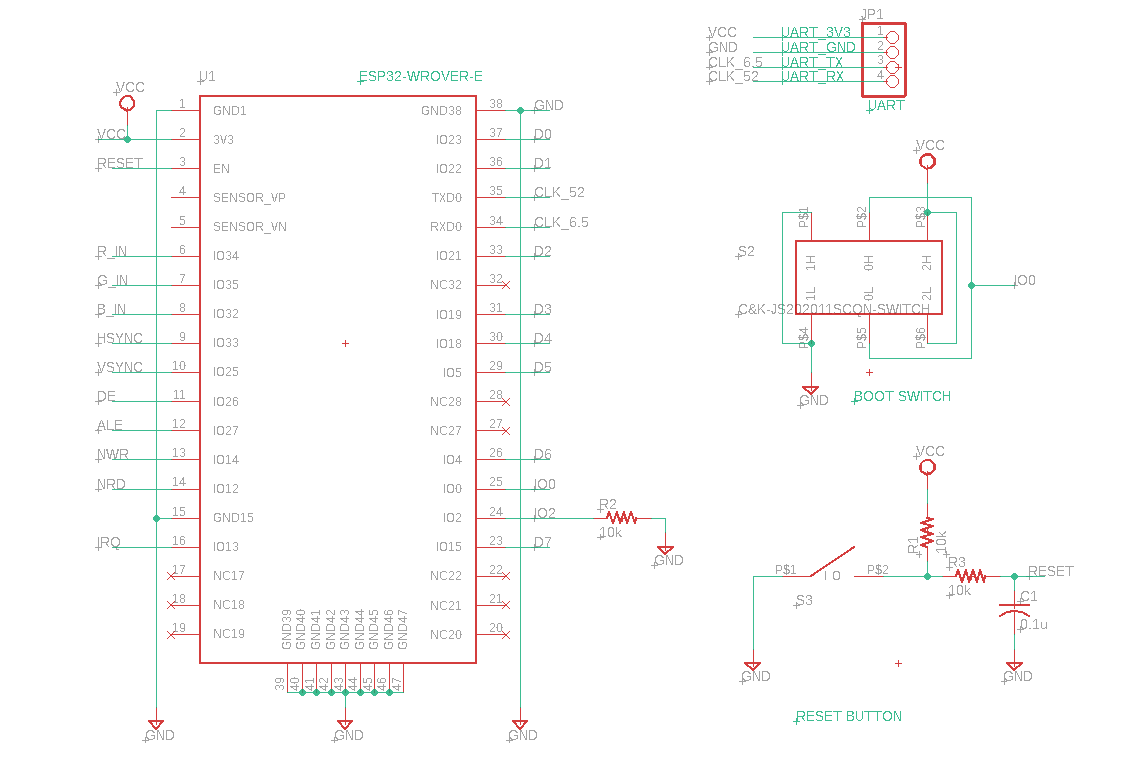
\includegraphics[width=0.95\textwidth]{comms_schem.png}
	\caption{Communication Subsystem Schematic}
	\label{fig:comms_schem}
\end{figure}

The schematic I designed for this subsystem is shown below in Figure \ref{fig:comms_schem}. The peripheral components include a boot switch, reset button, and UART header pins. The boot switch controls whether the MCU downloads the program from the UART interface of loads the progam saved in the flash memory on the module. The reset button is used to restart and reload the program on the MCU. A simple RC deboucing filter with time constant $\tau = RC = 1ms$ is included to prevent multiple resets from a single press. A simulation showing the effect of this debouncing is shown below in Figure \ref{fig:debounce}. Finally, a single pull-down resistor is used with the IO2 port of the MCU. The UART download boot mode relies on this logic value on IO2. The control components and many component values included in this schematic have been chosen from the instructions provided in the ESP32-WROVER-E Datasheet \cite{wrover}.

\begin{figure}[!h]
	\centering
	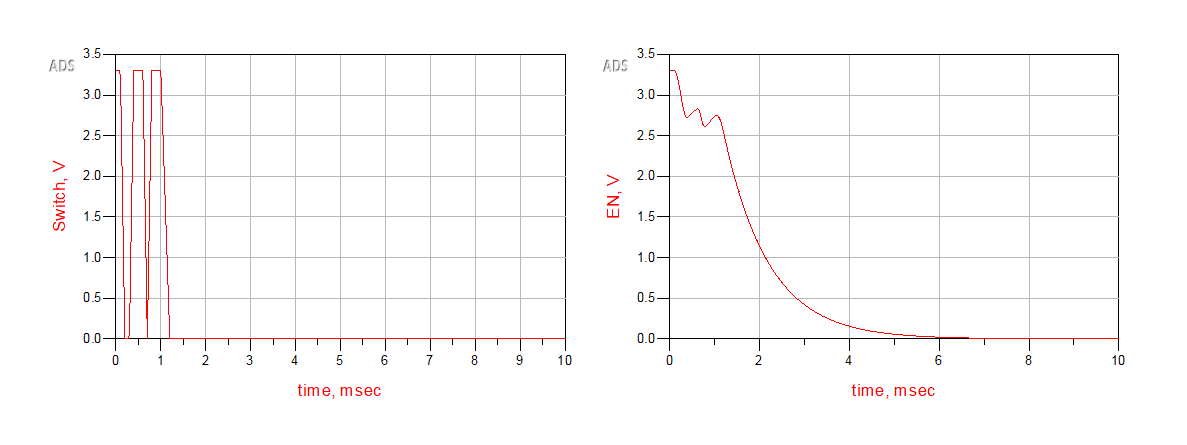
\includegraphics[width=0.95\textwidth]{reset_debounce.png}
	\caption{Reset Button Debouncing Simulation}
	\label{fig:debounce}
\end{figure}

This subsystem has direct hardware connections to the power, card reader, and display subsystems. The power subsystem provides the 3.3V source at all points in the schematic labeled VCC. The GPIO pins labeled R\_in, G\_in, B\_in, HSYNC, VSYNC, DE, CLK\_52, CLK\_6.5 are all used to control the display subsystem. The GPIO pins labeled ALE, NWR, NRD, IRQ, and D0-7 are used to control and receive card interrupts from the card reader subsystem. How these subsystems are controlled by the MCU firmware is handled by the respective subsystem.

\subsection{Display Subsystem}

The primary component in the display subsystem in the 3.5 inch LCD display. This display is a color 320x240 pixel display and controlled through a 24-bit RGB input. This particular display was chosen as a full color screen on the device is much more visually appealing than a text display or a thin black and white display. Along with the LCD are three shift registers used to convert the 24-bit parallel input into 3 serial inputs for use by the MCU. This allows for the same control of the LCD with a higher clock requirement and without using 24 separate GPIO pins. The schematic designed for this subsystem is shown in Figure \ref{fig:disp_schem}. The hardware wiring of this subsystem is simple, the majority of the control work will be within the MCU firmware in creating a system that can maintain the 52 MHz serial rate for each color. The chosen MCU has a CPU clock of 240MHz as specified in the ESP32 Technical Reference Manual \cite{esp32_tech} indicating that it should be able to handle these operations. All of the pin specifications and clock requirements for the LCD have been acquired from the LCD Datasheet \cite{orient_lcd}.

\begin{figure}[!h]
	\centering
	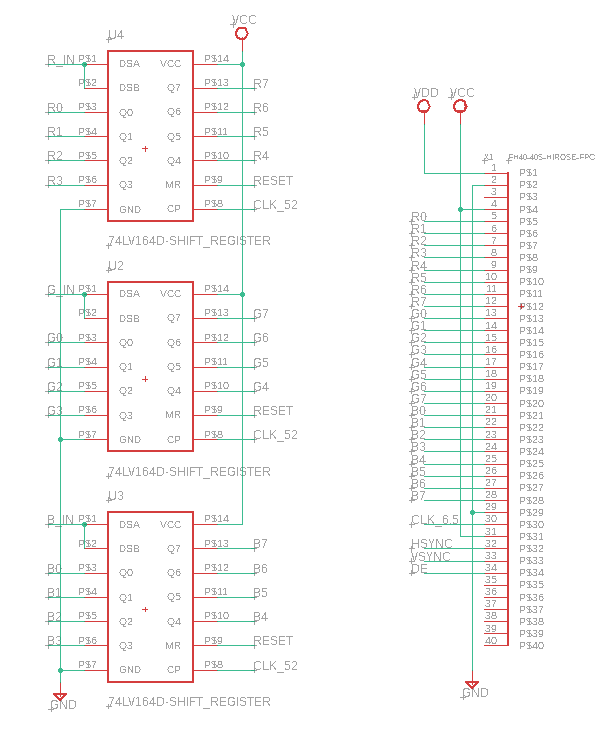
\includegraphics[width=0.75\textwidth]{disp_schem.png}
	\caption{Display Subsystem Schematic}
	\label{fig:disp_schem}
\end{figure}

This subsystem connects to the communications and power subsystems. The communications subsystem provides the control input through the R\_in, G\_in, B\_in, HSYNC, VSYNC, DE, and clock signals. The power subsystem provides a 3.3V source at all points labeled VCC and a 9.6V source at all points labeled VDD. The reset button that is used with the MCU is also wired to the shift register reset pin to allow the shift registers to clear on the reset of the MCU. This should not matter as each pixel color value will fully overwrite the shift register contents.

The layout with necessary footprints I created for the combination of the communications and display subsystems is shown below in Figure \ref{fig:layout}. The remainder of the layout was created by other memebers of the group.

\begin{figure}[!h]
	\centering
	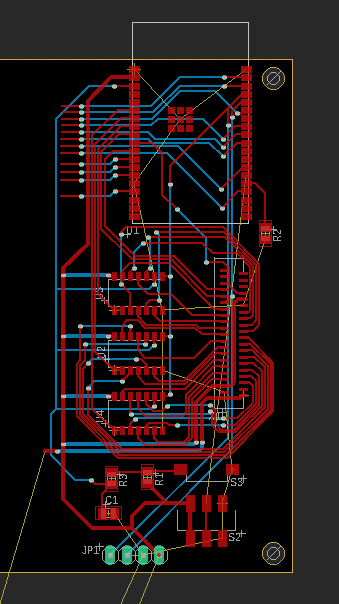
\includegraphics[width=0.45\textwidth]{layout.png}
	\caption{Communication and Display Subsystem Layout}
	\label{fig:layout}
\end{figure}

\subsection{Power Subsystem}

The power subsystem is composed of a battery with built in protection circuitry, a low drop-out linear voltage regulator to provide the 3.3V source, a boost converter to provide the 9.6V source, and a buck converter to convert from a 5V USB input to the optimal 4.2V charging voltage specified by the battery. The USB charging input is a micro-USB port and was chosen due to it being a very common charging method for small devices. The battery was chosen from a simple calculation of the peak current draw for each major component in the system and required a peak discharge current of just under 1A. Lastly, a switch is provided to choose between, the off state, the on state, and the charging state.

\begin{figure}[!h]
	\centering
	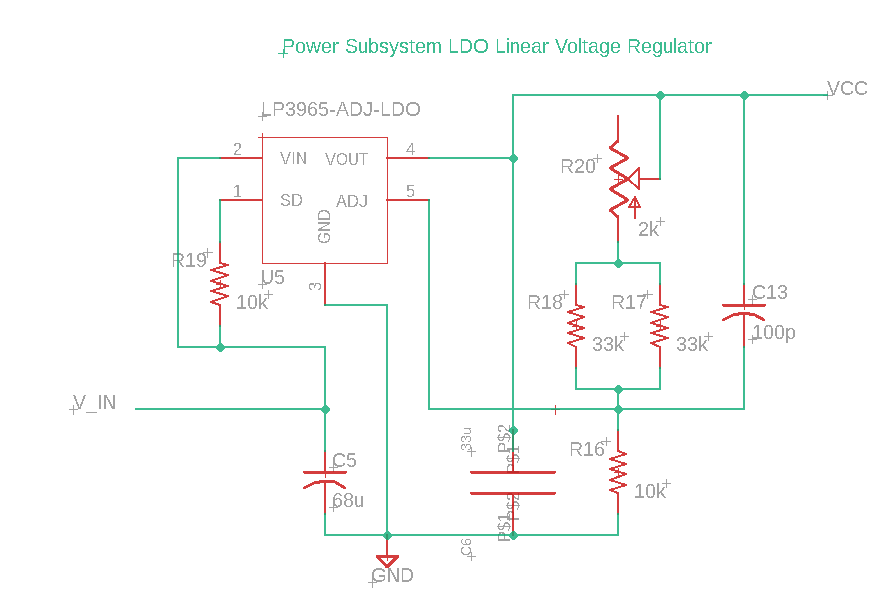
\includegraphics[width=0.85\textwidth]{ldo_schem.png}
	\caption{Power Subsystem Linear Voltage Regulator Schematic}
	\label{fig:ldo_schem}
\end{figure}

The schematic designed for the linear voltage regulator is shown in Figure \ref{fig:ldo_schem}. The chosen component is adjustable to allow for tuning of the output voltage to 3.3V. The input and output capacitor and biasing resistor selection are dictated by the LDO Datasheet \cite{ldo}. R16 or R1 in the datasheet is set to $10k\Omega$. R2 is the combination of R18 and R17 in parallel with R20 in series. The exact value of R2 is calculated to be
\[ R2 = R1(\frac{V_{out}}{1.216} - 1) = 17.138k\Omega. \]
The implementation allows for a range from $16.5k\Omega$ to $18.5k\Omega$ to account for tolerances and imperfections in components.

\begin{figure}[!h]
	\centering
	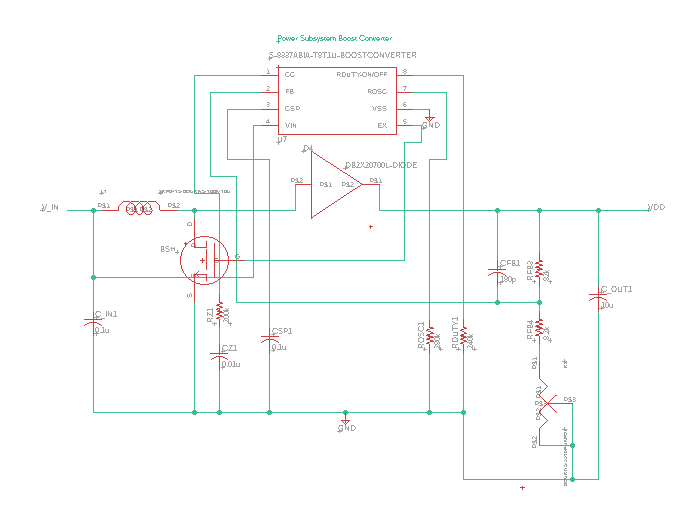
\includegraphics[width=0.95\textwidth]{boost_schem.png}
	\caption{Power Subsystem Boost Converter Schematic}
	\label{fig:boost_schem}
\end{figure}

The schematic designed for the boost converter is shown in Figure \ref{fig:boost_schem}. The main component is a boost switching controller meaning it provides the signals to an external MOSFET but the power does not run through the chip. This design method was chosen because of concerns over the complexity of our design but will lead to more chances for errors. A potentiometer is included with the biasing resistors again to allow for tuning of the output voltage to 9.6V. The input and output capacitor, inductor, MOSFET, and biasing resistors selection are dictated by the Boost Controller Datasheet \cite{boost}. Using the datasheet range, and inductor of $10\mu H$ and an oscillation frequency of 500kHz were choosen.This boost converter is used to power the LED backlight of the LCD. The LCD specifies an voltage of 9.6V and max current of 50mA. Assuming an efficiency of slightly less than 70\%, this corresponds to a max current of 210mA at 3.3V. The continuous mode peak current is then
\[ I_{PK} = \sqrt{\frac{2I_{out}(V_{out} + V_D - V_{in}}{f_{osc}L}} \approx 0.38A. \]
The required resistance for the chosen oscillation frequency is $280k\Omega$. To allow for a large maximum duty cycle and provide a wide range of available output voltages, the resistance chosen for the duty cycle is $240k\Omega$. The biasing resistors started with setting $R_{FB1}=82k\Omega$. Using $V_{out} = \frac{R_{FB1}+R_{FB2}}{R_{FB2}}$, $R_{FB2} = 9.5k\Omega$. The shown implementation allows for a range from $8.2k\Omega$ to $10.2k\Omega$.

\begin{figure}[!h]
	\centering
	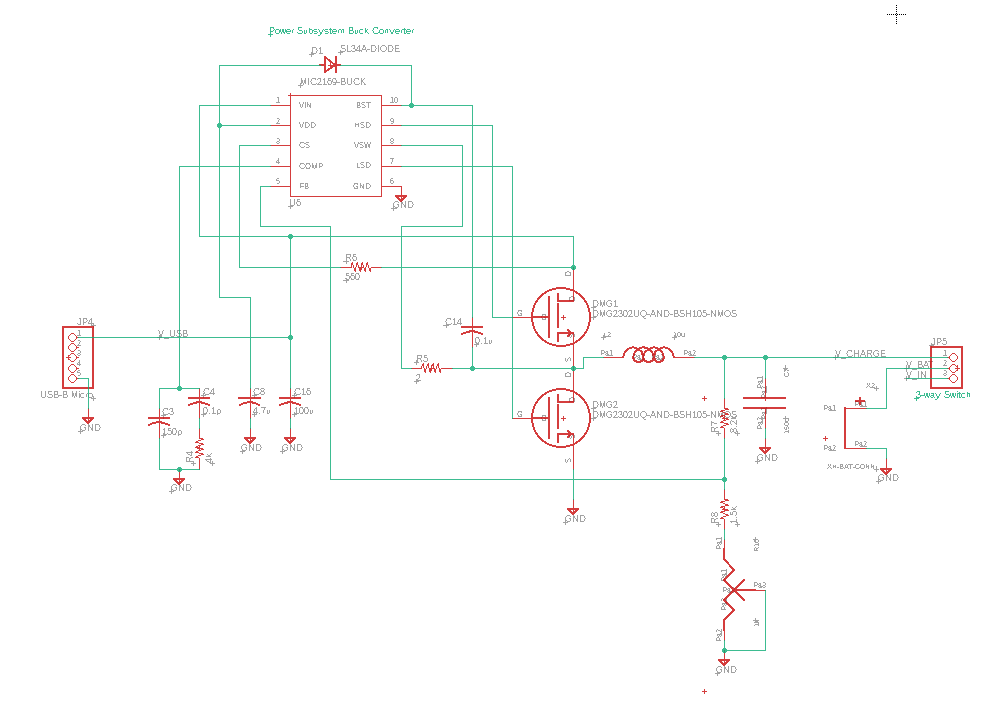
\includegraphics[width=0.95\textwidth]{buck_schem.png}
	\caption{Power Subsystem Buck Converter Schematic}
	\label{fig:buck_schem}
\end{figure}

The schematic designed for the buck converter is shown in Figure \ref{fig:buck_schem}. This is also a switching controller implementation chosen for the same reasons as the boost converter. The component selection was dictated by the Buck Controller Datasheet \cite{buck}. The buck converter must be able to handle a maximum output current of 2A. The chosen MOSFETs have a drain-source resistance of $35m\Omega$ when on. From the datasheet, the inductor was chosen to be
\[ L = \frac{V_{out}(V_{in} - V_{out})}{0.2V_{in}f_{osc}I_{out(max)}} \approx 3.3\mu H. \]
The ripple current in the inductor can then be determined to be
\[ I_{ripple} = \frac{V_{out}(V_{in} - V_{out})}{0.2V_{in}f_{osc}L} \approx 0.4A. \]
The recommended current limit for the device is thus
\[ I_L = I_{load} + \frac{1}{2I_{ripple}} = 3.25A. \]
This limit can be set by choosing
\[ R_{CS} = \frac{R_{DS,on}}{200\mu A}I_L \approx 560\Omega. \]
The voltage selection includes a potentiometer to allow for the tuning of the output voltage. The R1 from the datasheet is implemented as R7 in the schematic and is chosen to $8.2k\Omega$. R2 can then be calculated as
\[ R2 = \frac{0.8R1}{V_{out} - 0.8} \approx 1.93k\Omega. \]
The implementation shown allows for a range of $1.5k\Omega$ to $2.5k\Omega$.

As previously mentioned, this subsystem was originally not my responsibility, I did the work to attempt to meet deadlines for the project. That being said, I do not plan on taking the future power subsystem responsibilities for the remainder of the project.

\subsection{App Subsystem}

The programming of the app can be done largely independently of the rest of the project. I have begun planning out the method of programming, but have not written physical code to this point. Originally, the app was to be implemented on an Android device. We were not able to borrow one from the ECE department so we had to look into other methods. We could attempt an IOS app, but this requires Apple computers for development which would put the burden of app development entirely on a single member of the team. Instead it was decided to create a computer app as this will be accessible in development to all members and will still meet all the requirements specified in the design document.

I have decided to use C++ for the creation of the app due to the many libraries that exist to help with low level graphics and Bluetooth connection. Additionally, from my experience in creating Android apps, C++ can be implemented into the Android apps fairly easily making it a good proof of concept for a phone app if this product were taken to full development. The main other option for this development would have been Java, but C++ was decided based on our team's experience. I have chosen the SFML library for the graphics due to its simplicity and available documentation. I plan on using Windows sockets for the Bluetooth implementation because it also has many resources and examples available.

\section{Verification}

Due to shipping delays, construction and testing of the device has not started. The following section will outline tests that I will perform for these subsystems.

\subsection{Communication Subsystem}

The main requirement of the communication subsystem is to be able to accurately deliver information to the app via Bluetooth. To test, a simple program will be uploaded to the MCU via the UART pins that contains the Bluetooth sending and receiving functionality and a sample file of size 5kB. The PCB will be placed 3 feet away from the receiving device. The MCU will link with the device and send the file. The total time to receive the file will be recorded by the receiving device starting from the time at which the two devices established a Bluetooth connection. The contents of the transmitted file will be checked against the original for accuracy and the total time will give a general idea of the throughput of the system.

\subsection{Display Subsystem}

The first requirement of the display subsystem is for the MCU to meet the clocking requirements. This will be tested by uploading a simple program to the MCU to establish the desired clock rates at pin 34 and 35 of 6.5MHz and 52MHz respectively. These pins will then be probed with an oscilloscope to verify the switching frequencies.

The next output will be on the MCU's capability to output data properly and at these specified speeds. A similar setup will be created to the previous test. The program loaded to the MCU will now have pins 6, 7, and 8 (RGB in pins) output data serially based on a value in memory. That memory value will be set to 0xAA so that the pin output will change value at each clock edge. Probes will be used from the oscilloscope to verify this behavior. This test will confirm the MCU's ability to read from memory and output the data at the needed speeds.

\subsection{App Subsystem}

The portion of the app which I am responsible is the Bluetooth portion. Thus the testing that I will do for the app subsystem will involve a ``Hello World!'' type test. The throughput of the device does not need to be tested as the central device will likely create more of a bottleneck than the app and the throughput has already been tested once. To verify that communication is available in either direction, the app will create a hello world packet. The MCU will be loaded with a program to receive the packet and send an acknowledgment if the contents matches what is expected. The app will need to receive this acknowledgment to pass the test confirming accurate communication in both directions.

\section{Conclusion}

\subsection{Timeline}

The general timeline for the completion of the construction, testing, and coding is outlined in the Schedule within the Design Document. For construction, this is dependent on the arrival of some parts, but I would like to have this completed for myself and all members of the team by the end of next week. Along with this, I would like to finish firmware programming and testing within the next two weeks. For the app development, the initial development will be done this week but will not be finalized until after the other pieces of the project are completed. With this plan, I will have an extra week before the demonstrations begin for any final testing and system debugging.

\subsection{Ethics and Safety}

Much of the ethical consideration of the project surrounds gambling and cheating. We avoid this by constructing the device in a way such that it would not be able to be used discretely in any professional setting. Additionally, the system uses only information already available to the player when informing on game status and individual hand information or suggestions. These ethical considerations have been discussed fully previously in the Design Document.

This project fully follows the IEEE Code of Ethics \cite{IEEE_ethics}. This project does not present any harm to players are general public. The only source of potential harm would be through the radio frequency communication but the NFC signals at 13.56MHz and Bluetooth signals at 2.4GHz are within the typical range of frequencies and have no evidence of causing any health issues. This project also does not have any forms of harassment or discrimination that can be seen. This project also follows the Bluetooth Code of Conduct \cite{BT_conduct} as it does not transmit an harmful content or transmit excessive amounts of data.

Any electrical project has its safety concerns often from the high power or high current considerations. All components selected for this device within the power subsystem have been specifically chosen with current and voltage ratings in mind. Each member of the team, myself included, has read the ECE 445 Safety Guidelines \cite{445_safety} and completed the necessary training for the lab. This device uses a Lithium Ion Battery which comes with safety considerations as specified in the ECE 445 Safe Practice for Lead Acid and Lithium Batteries \cite{Li_safety}. These safety considerations have been read and are being followed for all activities involving the battery. Lastly, the project will be enclosed in a non-conductive casing to protect all users from any electrical malfunctions.

% Bibliography (references in separate file)
\bibliographystyle{IEEEtran}
\bibliography{references.bib}

\end{document}
